\documentclass{article}
\usepackage{graphicx} 
\usepackage{subfigure} 
\usepackage{natbib}

\usepackage{algorithm}
\usepackage{algorithmic}

\usepackage{amsthm}
\usepackage{amsfonts}
\usepackage{amssymb}
\newtheorem{mydef}{Definition}

\usepackage{listings}
\usepackage{color}

\definecolor{dkgreen}{rgb}{0,0.6,0}
\definecolor{gray}{rgb}{0.5,0.5,0.5}
\definecolor{mauve}{rgb}{0.58,0,0.82}

\lstset{frame=tb,
  language=Python,
  aboveskip=3mm,
  belowskip=3mm,
  showstringspaces=false,
  columns=flexible,
  basicstyle={\small\ttfamily},
  numbers=none,
  numberstyle=\tiny\color{gray},
  keywordstyle=\color{blue},
  commentstyle=\color{dkgreen},
  stringstyle=\color{mauve},
  breaklines=true,
  breakatwhitespace=true
  tabsize=3
}

\usepackage{hyperref}

\usepackage{amsmath}

\newcommand{\theHalgorithm}{\arabic{algorithm}}
\usepackage{icml2013} 
\icmltitlerunning{Deep Q Network an Approach for General Agent Control}

\begin{document} 
\twocolumn[
\icmltitle{Deep Q Network\\ 
           an Approach for General Agent Control}
\icmlauthor{Yuan Gao}{yuan.x.gao@helsinki.fi}
\icmladdress{Department of Computer Science,
            P.O. Box 68 (Gustaf Hällströmin katu 2b) FI-00014 UNIVERSITY OF HELSINKI FINLAND}
% You may provide any keywords that you 
% find helpful for describing your paper; these are used to populate 
% the "keywords" metadata in the PDF but will not be shown in the document
\icmlkeywords{Deep Learning, Q Learning, Atari Game}
\vskip 0.3in
]
\begin{abstract} 
Deep Reinforcement Learning(DRL) is a method that combines deep learning and reinforcement learning. It was recently developed for control problems that needs to extract information from natural information such as images and voices. In this paper, we consider a DRL algorithm called Deep Q Network(DQN) to perform a learning task on atari game environment. Our discussion will mainly focus on the algorithm's background, motivation and implementation. By comparing with the other algorithms, this algorithm is able to show the how the algorithm outperforms other algorithms for same task. In the end, we will shortly point out differences between original algorithm and our own implementation of the algorithm.
\end{abstract}
\section*{Introduction}
Reinforcement Learning(RL) is an area that studies how to map situations with actions\citep{barto1998reinforcement}. RL algorithms have been vary successful in the many fields including robotics \cite{kober2012reinforcement}, clinical trial \cite{kuleshov2010algorithms} etc. However, when it is applied to game agent control, general framework of RL suffers the curse of dimensionality. When the spaces of perception and control both become continuous, it is very hard to discretize the space properly. Even if we can discretize the spaces, it is still very hard to find a way of performing efficient policy gradient algorithms for large amount of states. 

Similar to image classification tasks,game agent control algorithm also needs to observe and process images. In recent years, one algorithm called Convolutional Neural Network(CNN) was suggested in 1998\cite{lecun1998gradient}. The CNN is a multi-layer neural network with one input layer, several hidden layers and output layers. As it can detect the features of an image automatically, it has been treated as a very important preprocessing step for agent control algorithms\cite{mnih2013playing}.

The combination of value-function-based RL(i.e. a RL algorithm works by learning a action-value function\cite{barto1998reinforcement}) and CNN can be considered as relatively efficient agent control algorithm. On one hand, the RL algorithm part provides the entire analysis framework including mathematical modelling and optimization techniques. On another hand, the CNN part reduces the dimensions of input images. 

The organization of this paper is as follows. We first introduce the problem that we would like to solve. After that we take previous lines of analysis one step further in Section 2 and 3 by introducing value-function-based RL and CNN which form the foundation of our algorithm. In Section 4, we will combine these methods and introduce the algorithm Deep Q Network(DQN)for our problem. Results are shown in Section 5. We gather some statistics for performance of this algorithm. Conclusions are drawn in Section 6. 

\section{Problem Definition}
We would like to develop an AI agent that can play games automatically. Naturally, it evolves two things. One of them is the testing bed and another one is algorithm for controlling the agent. In the field of agent control, these have been classified as problem of perception and problem of control. In the following text, we first introduce the background knowledge of the Atari Learning Environment(ALE) and then we take the explanation further to the detail of the algorithms.

The Atari video games was release in year 1977. Selling for 30 millions consoles, Atari games are considered fun and successful. Now the Atari games are no longer commercial and widely used in the research area. Following this trend, a reinforcement learning platform ALE is established for the previous purpose in order to ease the engineering difficulty\cite{bellemare12arcade}. There are several reasons of testing on this environment. First of all, the environment provides several standard actions for agents. Simultaneously, the game offers the researchers a way to compare their work easily. Finally, the state of Atari games(i.e. combination of scree-shots and RAM states) is relatively easy to be observed and analysed. Each frame of game is just a 160 x 210 matrix and its RAM is only 128 bytes. It is simple enough for modern computer with high-frequency CPU to deal with.

The ALE provides an object-oriented framework for testing different agents on different games. The Figure~\ref{atari_game} shows several games supported by the ALE.  It shows the ALE is a very general testing environment and the experience is comparable with other algorithms.
\begin{figure}[h!]
\centering
{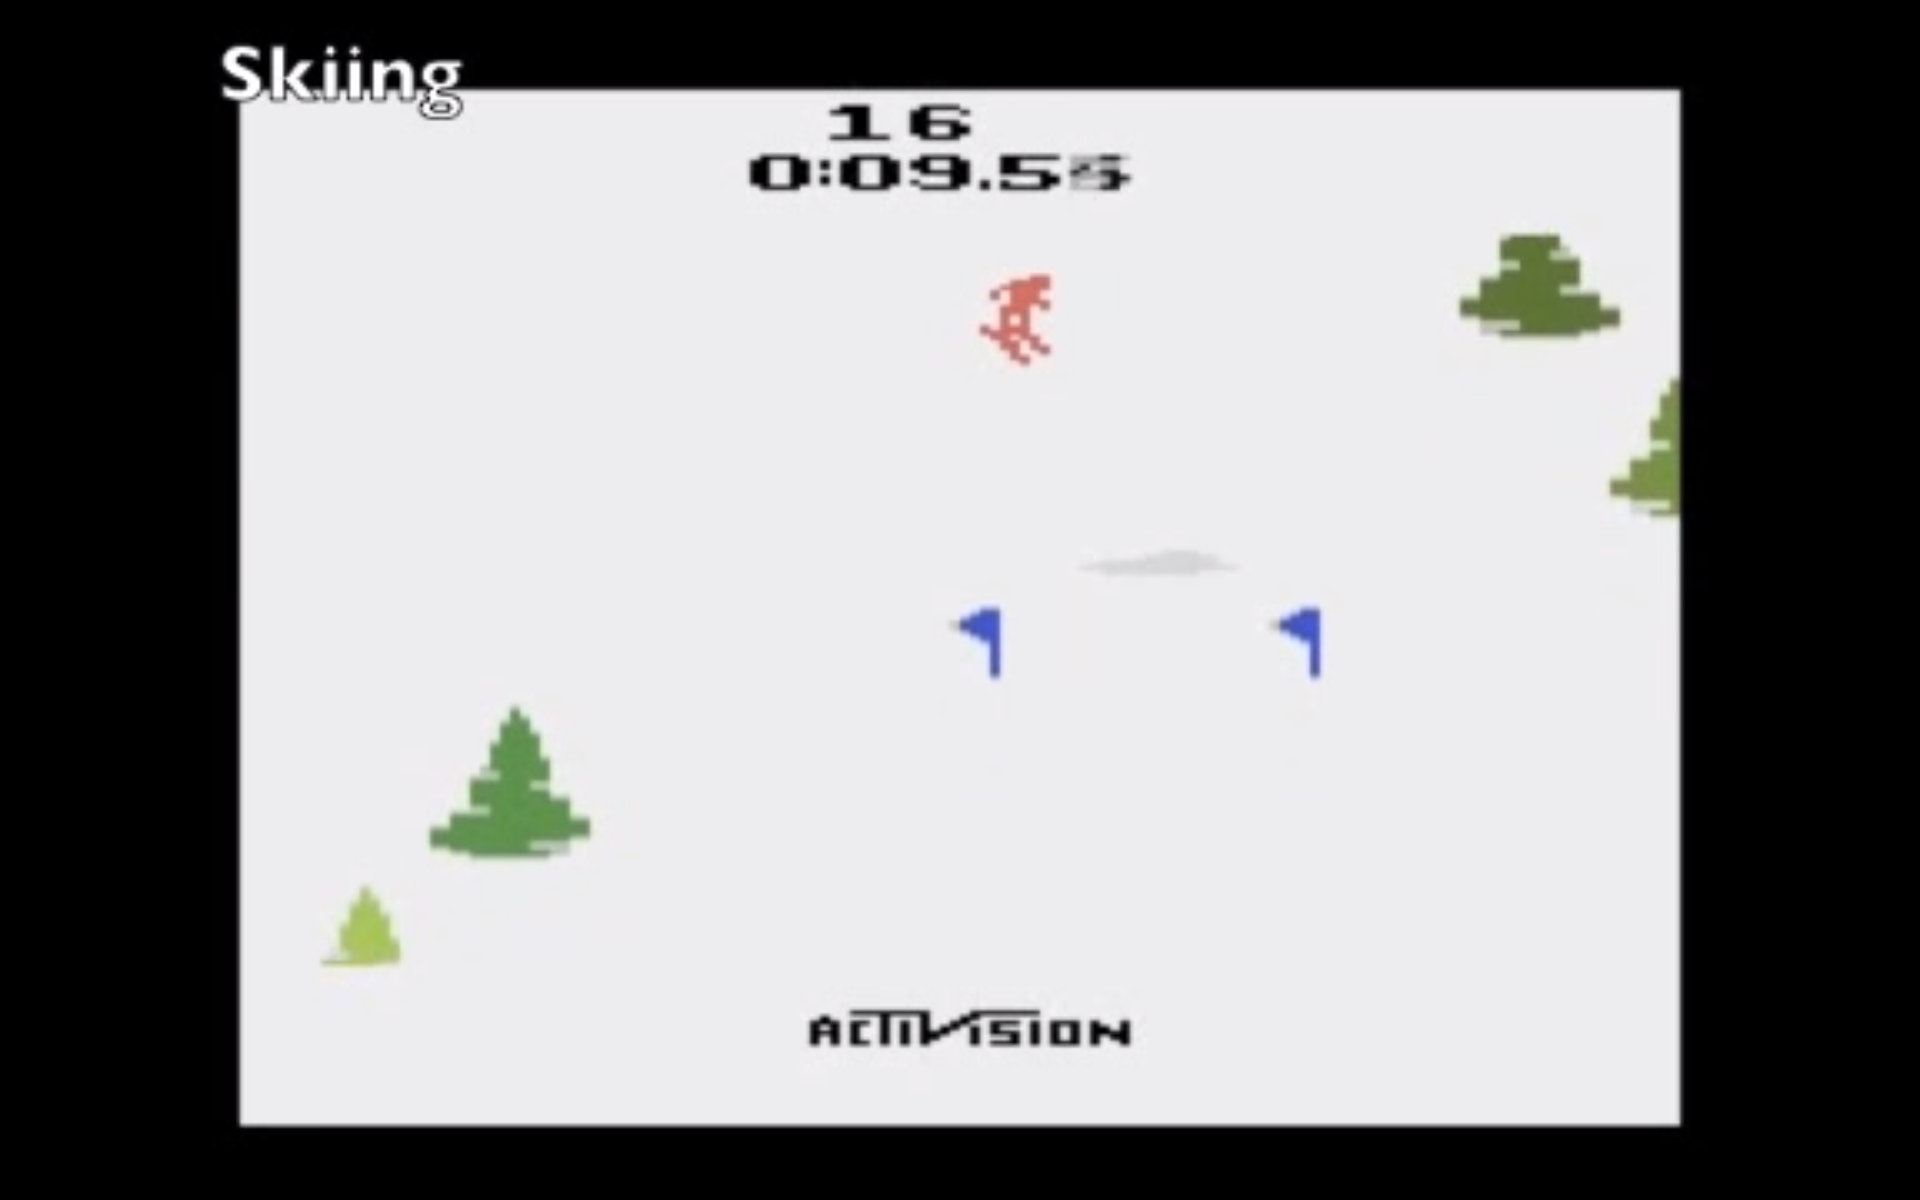
\includegraphics[width = 0.23\textwidth]{1}} 
{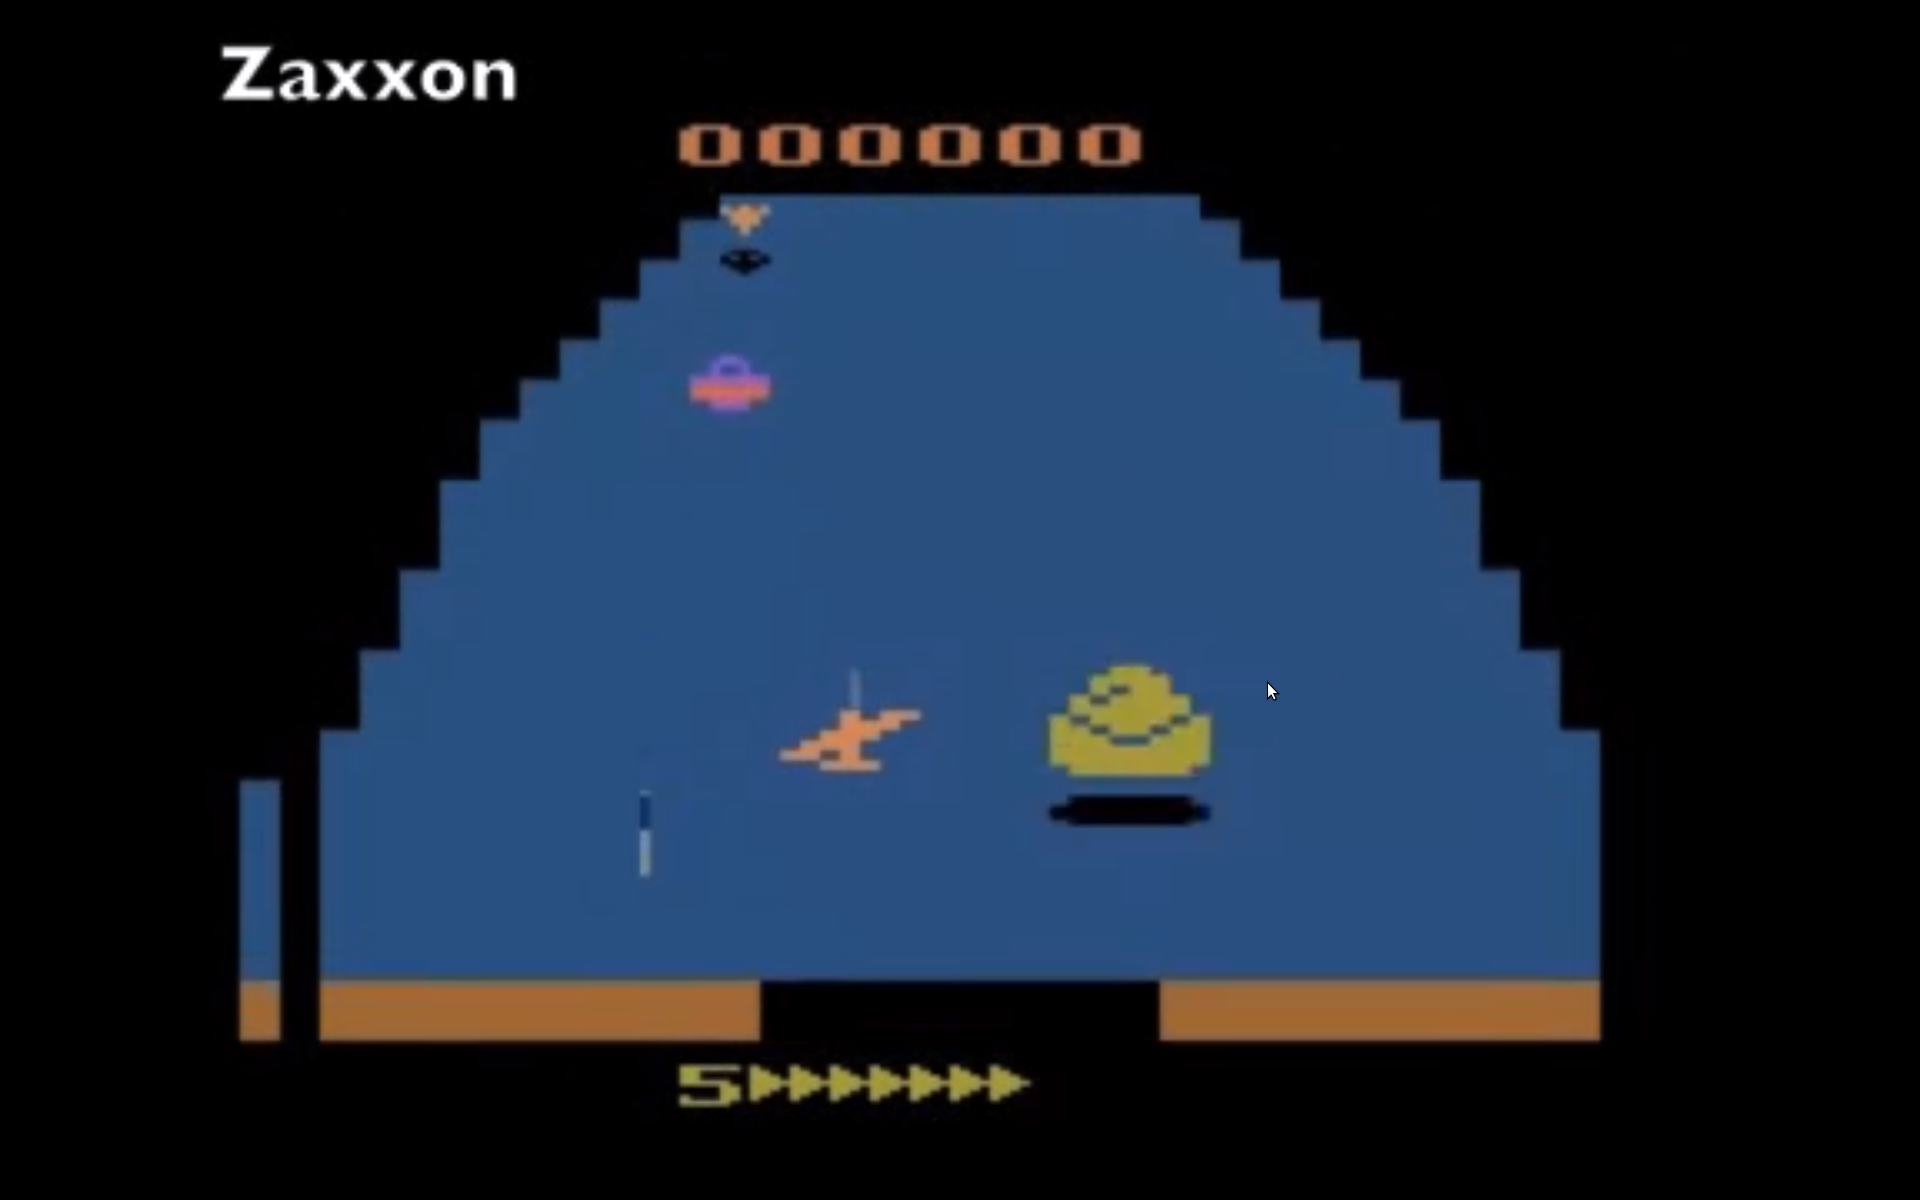
\includegraphics[width = 0.23\textwidth]{2}}\\
{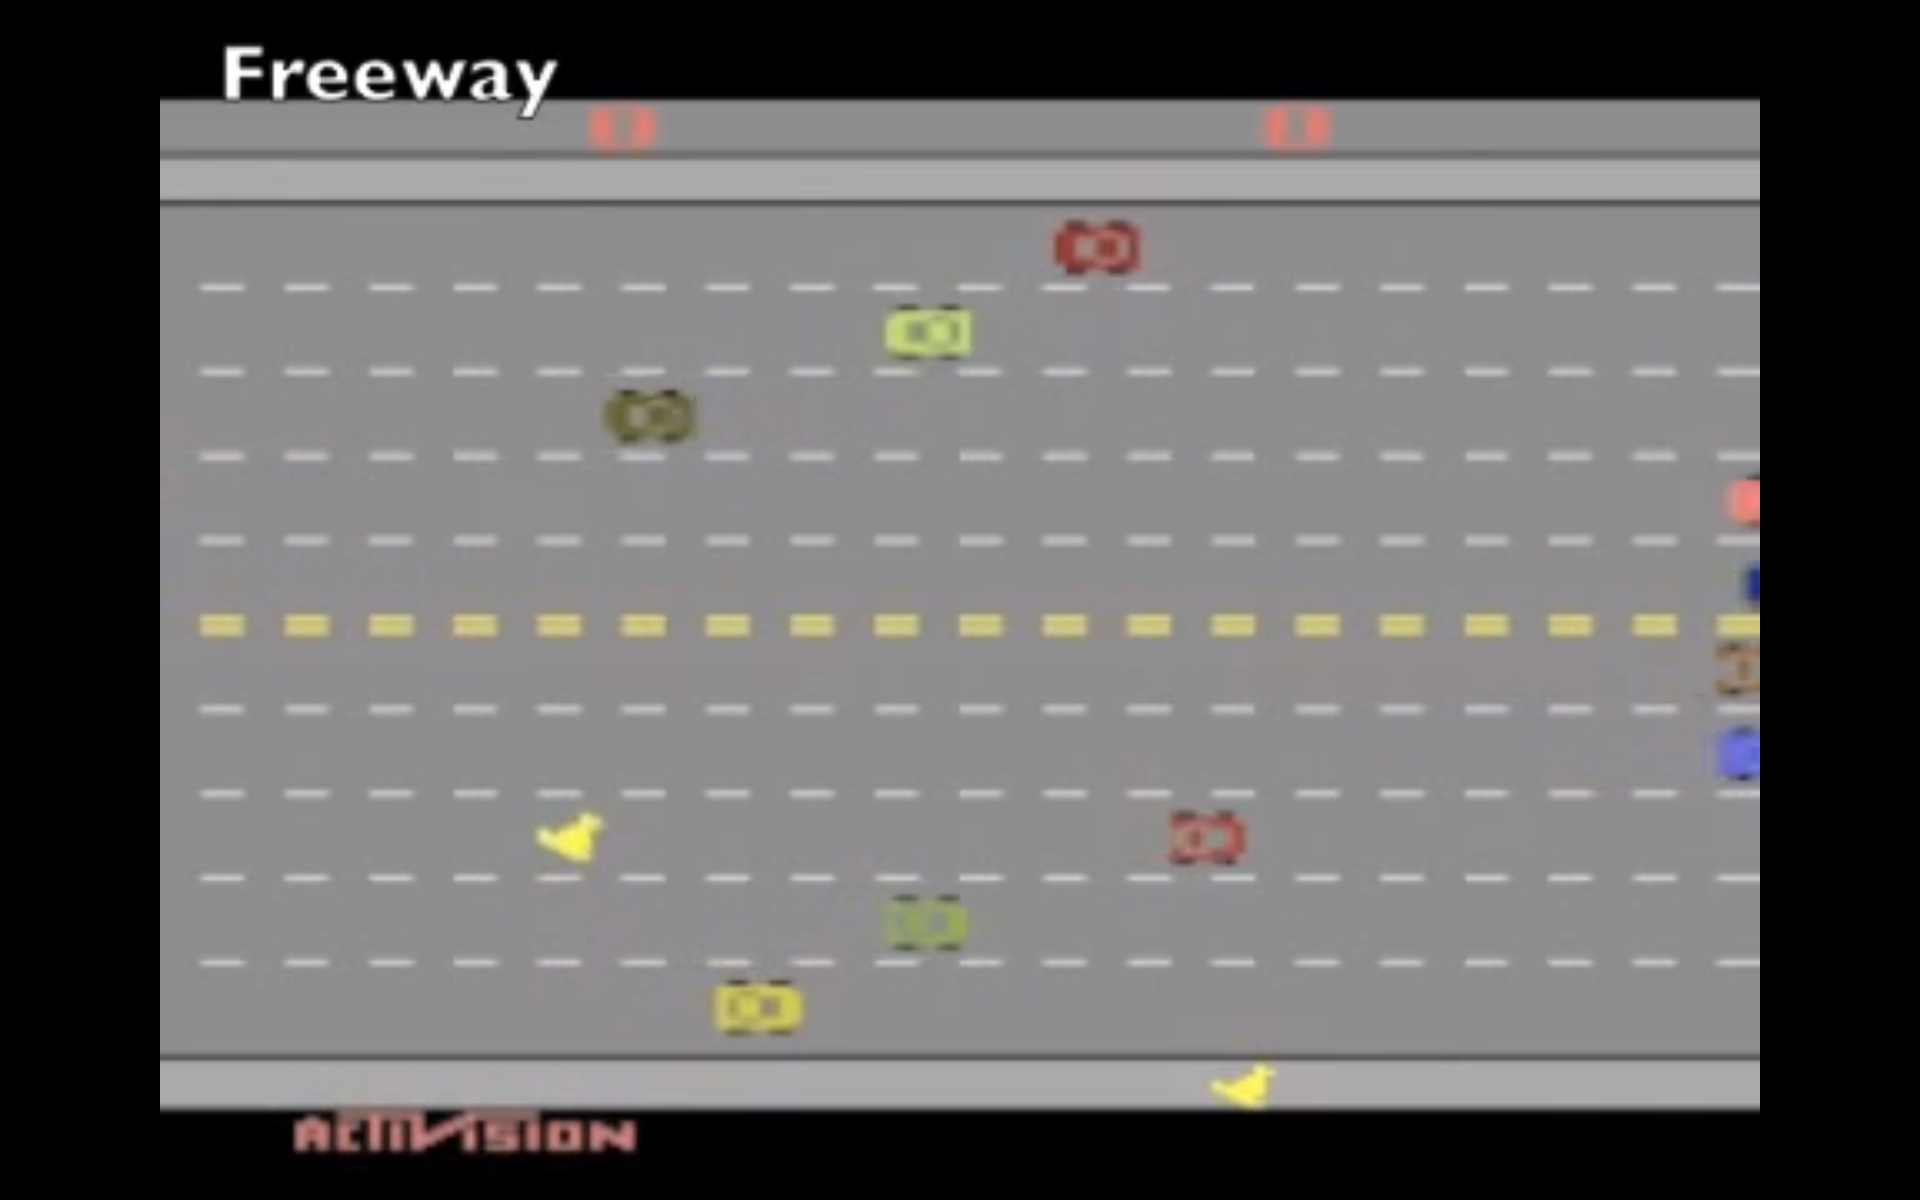
\includegraphics[width = 0.23\textwidth]{3}}
{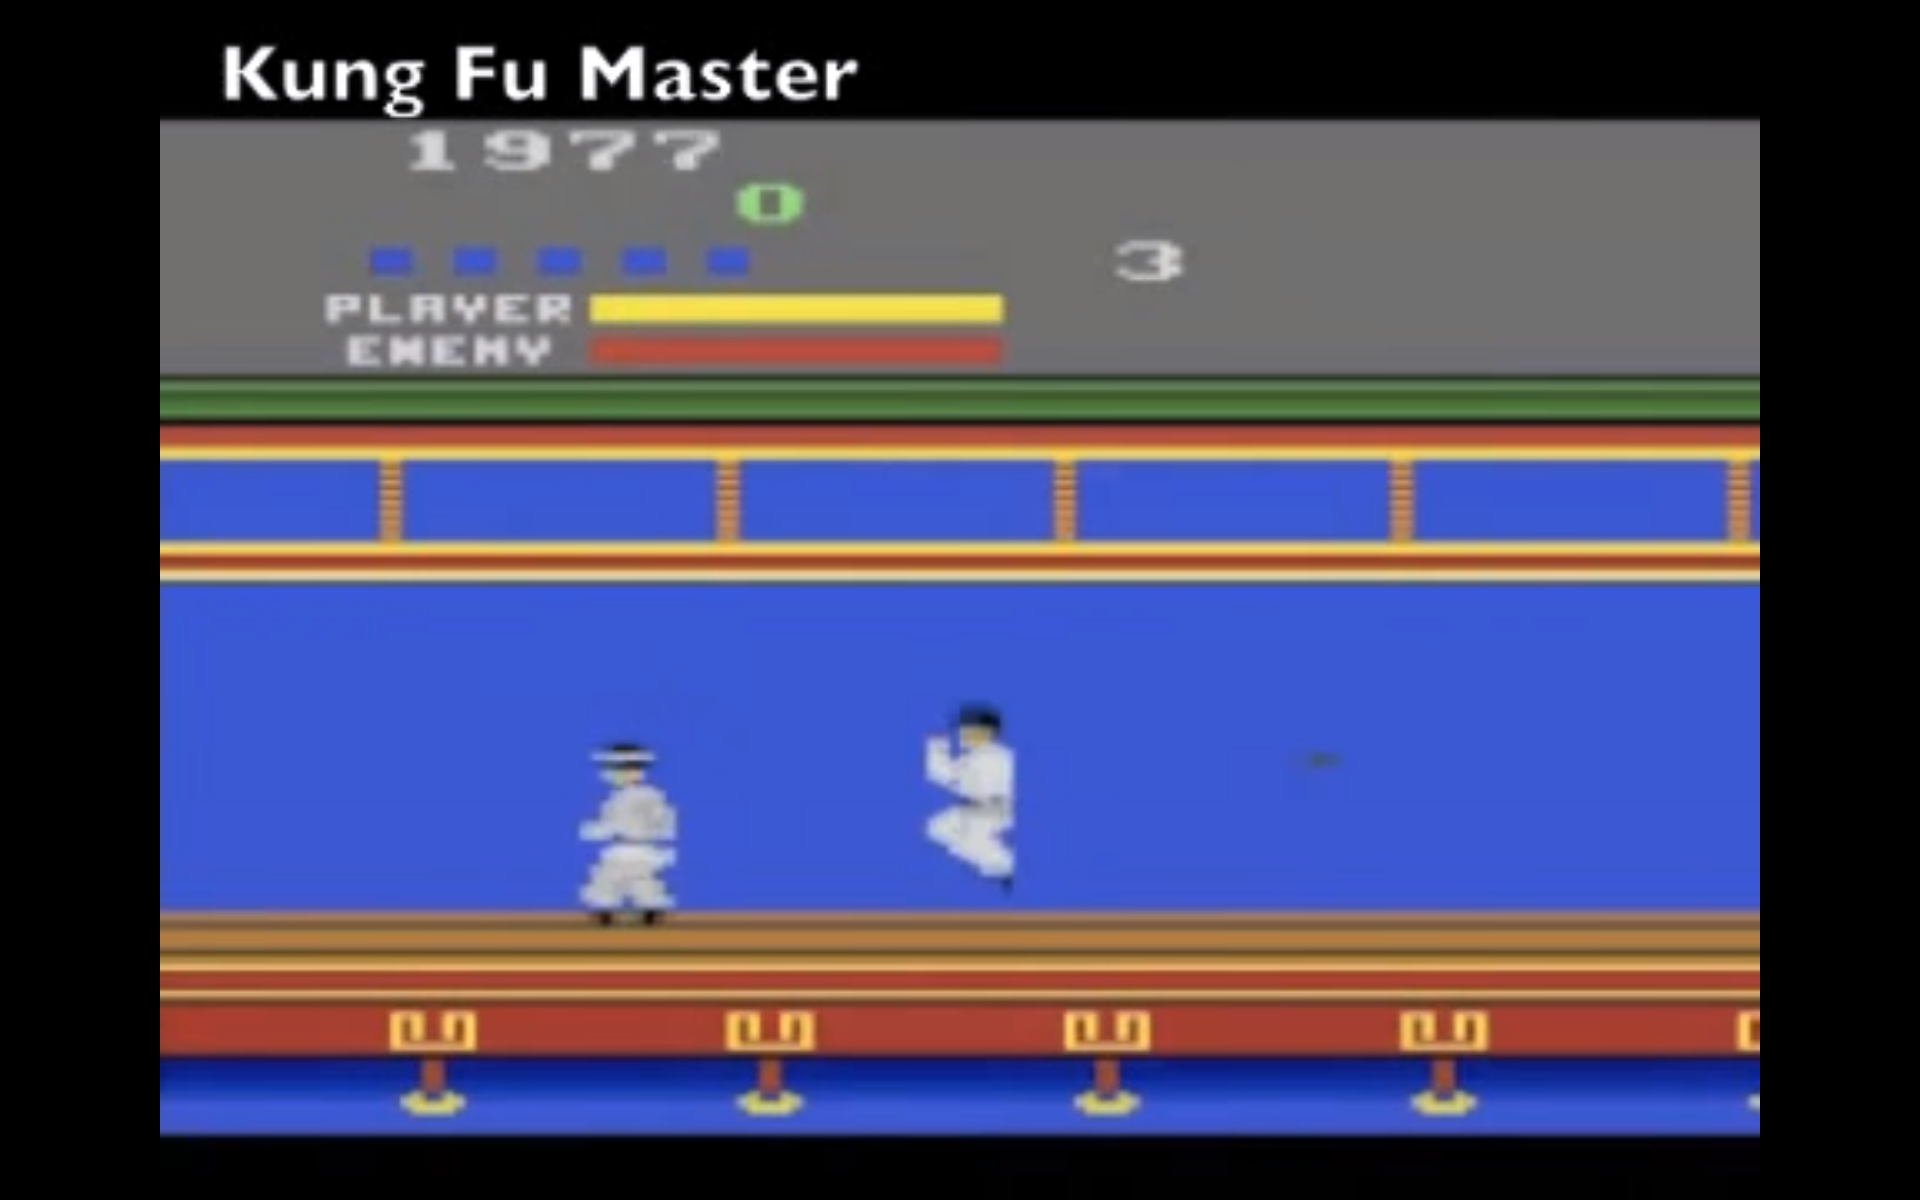
\includegraphics[width = 0.23\textwidth]{4}} 
\caption{This figure shows the basic games of the Atari Learning Environment(ALE) of reinforcement learning research. The upper left corner is famous atari 2600 game Skiing. The upper right corner is Zaxxon. The lower left corner is Freeway. The lower right corner is KongFu Mater. These games are representatives of the testing environment.}\label{atari_game}
\end{figure}

Now after deciding the environment, two main problems of game agent control algorithms(i.e. perception and control) are right in front us. Perception has always been considered not easy. At the beginning, for the sake of reducing the difficulty in such kind of problem, people considered to use hard-coded features to develop system.  

The transnational feature extraction algorithms include Basic Abstraction of the ScreenShots (BASS), 	Detecting Instances of Classes of Objects(DISCO) and Console Memory Reading \citep{naddaf2010game}. These detection algorithms are considered successful in various applications. Soon the designers found out that they always need to have prior knowledges of the structure of games to process their screen images. After that people started to think to develop a mechanism to automate this process. Inspired by neocognitron\citep{fukushima1980neocognitron}, a newly advanced unsupervised feature detection method for image classification Convolutional Neural Network(CNN) is developed .

The original CNN(Figure~\ref{cnn}) is a feed forward neural network meant to deal with the image classification problem. After it was proposed in 1998, it has became the state-of-the-art algorithm in this field.  These kind of networks always contain an input layer, several hidden layers, several fully connected output layers. The hidden layers consist several times of combination of two sub-layers. First of them is convolutional layer and second of them is  down-sampling layer.

The convolutional layer uses several convolutional kernels(i.e. filters) to convolve through the image after which down-sampling layer reduces the size of each convoluted image. In standard CNN(LeNet-5), the algorithm processes images like this for two times. The CNN than use two full layers to classify them. Latter in the Section of deep learning, we will investigate the details of this algorithm.

The most-impressive testing of this algorithm is made based on a game called Breakout\cite{mnih2013playing} in which agent need to control a bar to reflect a ball to break out all the bricks on the top. There are two actions for controlling the bar i.e. moving left and moving right.

\begin{figure}[h!]
\centering
{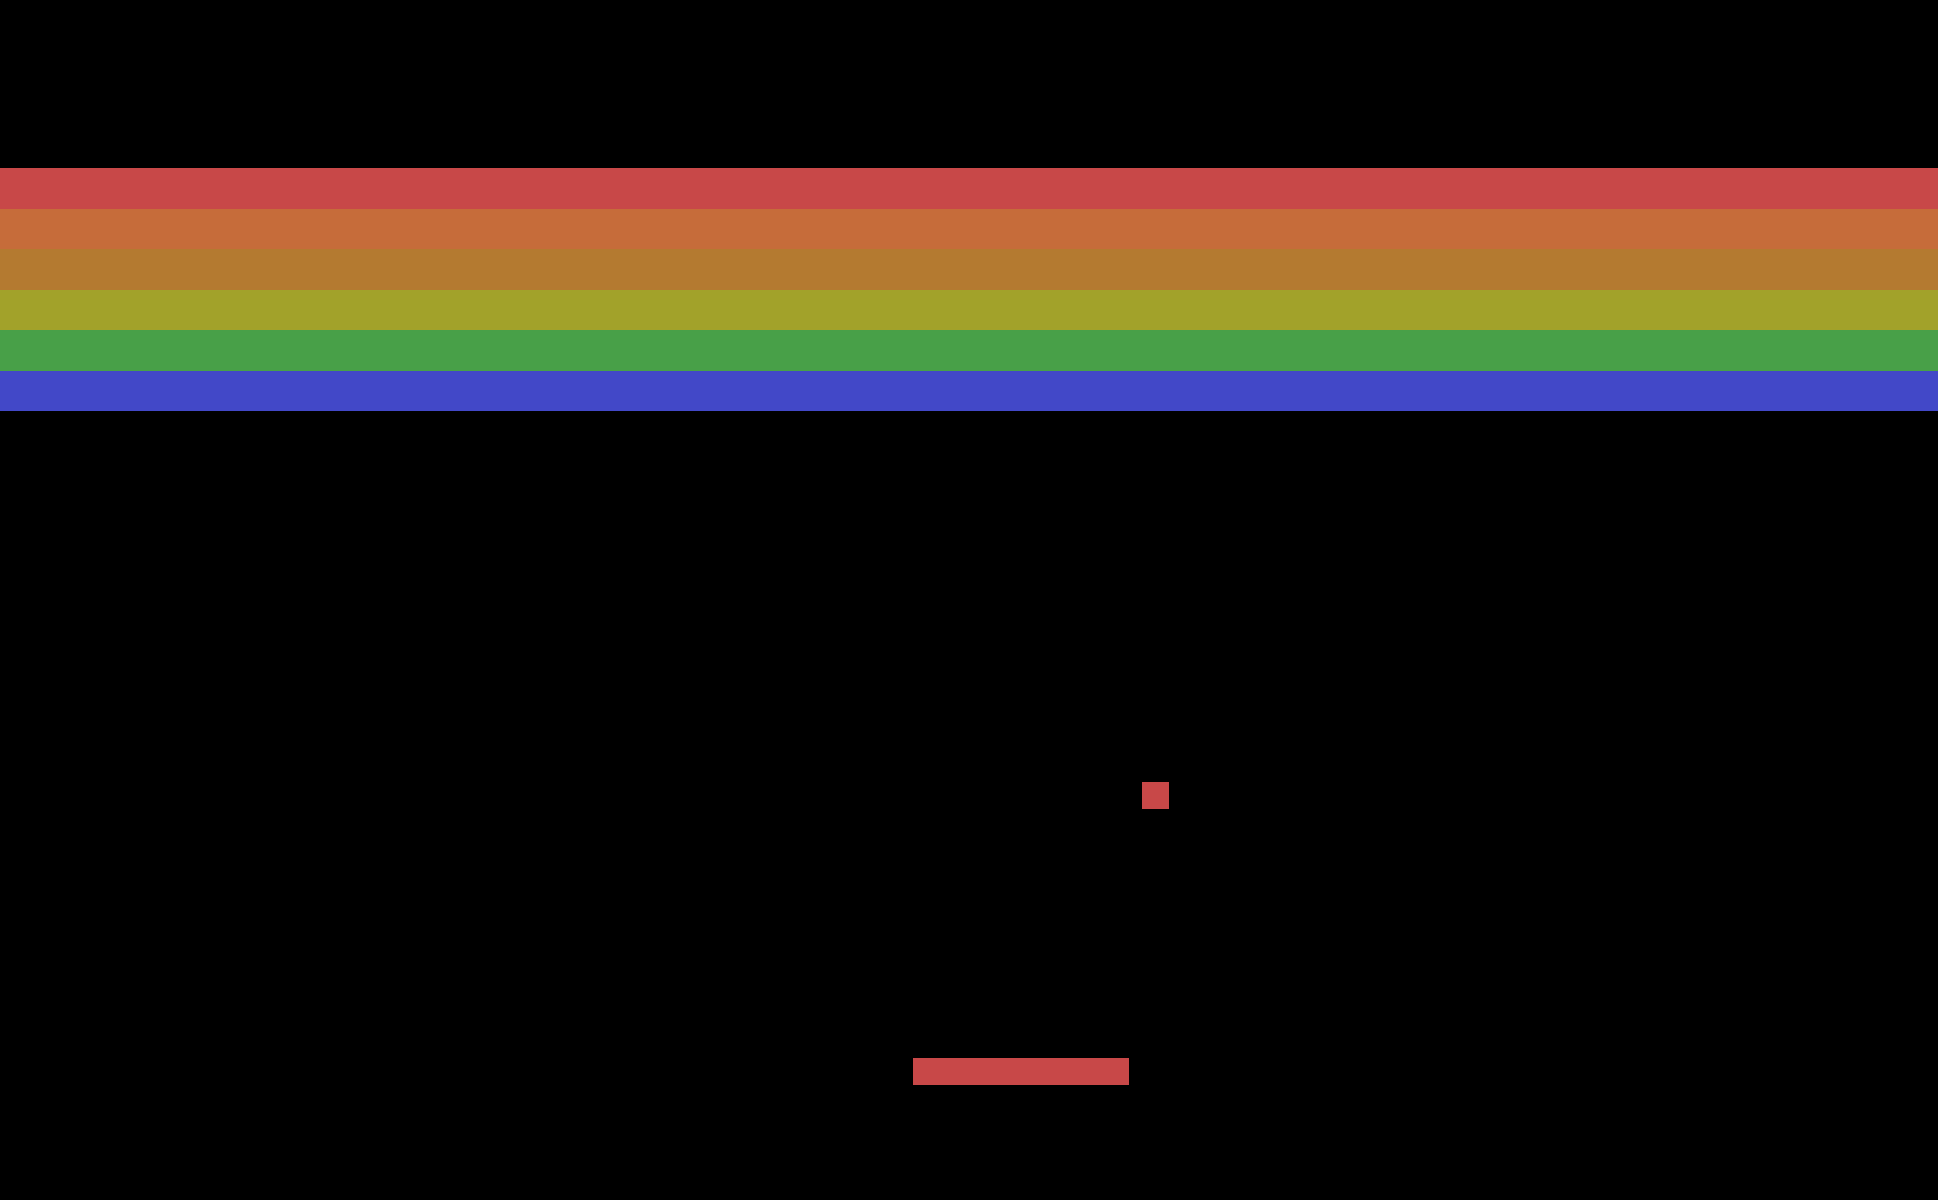
\includegraphics[width = 0.5\textwidth]{breakout}} 
\label{breakout}
\caption{This figure shows a typical process of game Breakout. In this figure, the agent is presented as a pink bar at the bottom. The white ball is used to break the bricks. The colourful bars on the top represent the bricks of the game. The goal of this game to break out all the bricks on screen. }
\end{figure}

\begin{figure*}
\centering
{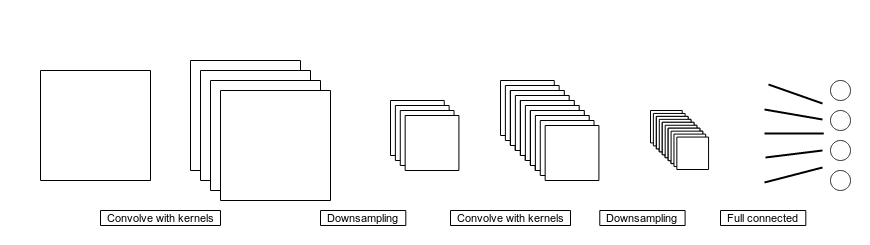
\includegraphics[width = 1\textwidth]{cnn}} 
\caption{This figure shows the structure of CNN, specifically LeNet-5 named after Yang LeCun. This CNN contains five layers of neural network including one input layer, two covolutional-downsampling layers, two full-connected layer. Along with the procedures showed in this figure, at beginning the image locally convolves with, normally, a 5x5 sliding matrix filter and generate several feature matrices. After the convolution, we use some way to down-sample the image. Normally some non-linear machanism(e.g. max-pooling) is used. The previous step ensures the important features are observed by the algorithm. As long as we get enough samples, a full-connected layer is then applied to classify them into lables.}\label{cnn}
\end{figure*}


\section{Reinforcement Learning}
In this section, we first give general intuitive concept of the Reinforcement Learning(RL) and then we formalize the problem of the reinforcement learning for the further description of the problem. To be precise, we will formalize the concepts of the Markov Decision Process, Policy and Reinforcement learning consequently.

If we would like to discuss what might be the most common way of learning, learning based on interacting with our environment is a natural idea to think about. When we were born in this world, we had no teachers around us. But tens of years passed, we learned to fear, to communicate with others and to write a paper. As a consequence, it is very natural to think that our environment is a great source of information. While playing around with environment, we learn by taking actions and getting reward from it. Now when we cook , when we do exercise, we are fully and acutely aware what will be the response of environment. 

The RL is an area that studies the mechanism of the such kind of learning in a computational way. Generally the goal of RL is to find a way of mapping different states with different actions so that we could maximize the reward signals. By definition, the RL is a big field. Because it at least contains computer science, psychology and philosophy.  Scientifically, its goal lies in discovering how people gain skills and practically, it gives the way of developing systems that can mimic the behaviour of human.

Unavoidably, the field of RL also has deep connection with machine learning field. In fact, it is one of three main areas in machine learning. The other two areas are supervised machine learning and unsupervised machine learning. They share certain properties. For example, all these methods require optimization algorithms to optimize objective function under some constrains. The RL, especially the value-function-based RL consists several main concepts including value function, policy and reward. Policy is the sequence of actions people would like to take to maximize reward. As a consequence, if we would like to find the best policy then we have to optimize process of policy iterations.
 
For better understanding of the Deep Q Network algorithm, we have to formalize several concepts in reinforcement learning. In the following text, we formalize the concepts of Markov Decision Process, Policy, Policy Value and the fundamental equation in RL- the Bellman's Equation.

\begin{mydef}
MDPs
A Markov Decision Process(MDP) is defined by a tuple $(\mathbb{S},\mathbb{A},T(.,.),R(.,.))$\footnote{In some definition, the initial state $s_0$ is added to the tuple.}
\end{mydef}
In the definition
\begin{itemize}
\item $\mathbb{S}$ is defined as set of states.
\item $\mathbb{A}$ is defined as set of actions.
\item $T(a,s)$ is the transition function that defines the transition distribution over all destination states. $s' = T(a,s)$.
\item $R(a,s)$ is the reward function that defines the transition distribution over all destination states. $r = R(a,s)$.
\end{itemize}
This probabilistic model is stochastic as the Markov property holds for both transition function and reward function.
\begin{mydef}
\textit{Policy}.
A Policy $\pi$ is an injection that maps state to action. $\pi:\mathbb{S}\rightarrow\mathbb{A}$
\end{mydef}
A policy is important for determining the so-called policy value. This value is used for finding the optimal policy as it is similar to a problem that try to find maximum value for all states.
\begin{mydef}
\textit{Policy Value}.
A policy value associated with a state $s \in \mathbb{S}$ is defined as a value $v_s(\pi) = V(s,\pi)$  where $v_s(\pi)  \in \mathcal{R}$. $V(s,\pi)$ represents the expected reward when the agent follows the policy $\pi$.
\end{mydef}
With a finite setting (i.e. finite states, finite actions, finite epoch $T$), $V(s,\pi)$  is defined as 
\begin{equation}
V(s,\pi) = \mathbf{E}\left[\sum_{i=0}^{T-t}\gamma^i r(s_{t+i},\pi(s_{t+i}))|s_t = s\right]
\end{equation}
Where $\gamma$ is the discount factor that ranges from 0 to 1.
\begin{mydef}
\textit{Bellman's equation}.
\begin{equation}
V(s,\pi) = \mathbf{E}\left[ R(s,\pi(s)) \right]+ \gamma \mathbf{E}\left[V(T(s,\pi(s)),\pi)\right]
\end{equation}\label{bellman}
\end{mydef}
Here we state the Bellman's equation without proof. This function determines an iterative update for the algorithm. Further information of proof can be found in Mohri's book called "Foundations of Machine Learning"\cite{mohri2012foundations}.

From Bellman's equation we can derive an iterative algorithm called Q-Learning algorithm. This algorithm is the first algorithm we could think about in reinforcement learning.~\ref{bellman}\citep{watkins1989learning}. Each iteration, the algorithm updates the expectation that algorithm can learn so far. Here we will shortly introduce the Q-Learning algorithm, as it plays a role in the Deep Q Network as well.

Q-Learning is a temporal difference RL algorithm i.e. an algorithm that uses the information contained in the difference of states over a short period of time. In fact, we do not need to specify any kind of model of environment. The algorithm is enough to extract the information from the environment based on using the reward function. 

The formula of the learning is as following.

\begin{align*}
Q(s_t,a_t) &\leftarrow Q(s_t,a_t) \\
	& + \alpha \left[r_{t+1} + \gamma \max_a Q(s_{t+1},a_t) - Q(s_t,a_t) \right]
\end{align*}

Where in this formula, the $\alpha$ is the coefficient that specifies rate of learning. If $\alpha$ is very large, the algorithm chose a greedier strategy. Otherwise the strategy is abstemious.

Literally, this formula would mean that, with a updating parameter $\alpha$, we update the value that corresponds the state if we take the optimal action. Optimal action is the one that can result to the maximum reward value.

To sum up, basically, we need to learn a value function $Q(s_t,a_t)$ to simulate the optimal policy $Q^*(s_t,a_t)$. If you notice, the above updating rule is very similar to the Bellman's equation and that is why we say this algorithm is derived from it.

\section{Deep Learning}
The deep learning recently has became a popular concept in the field of machine learning since 2006. Comparing with its opposite - shallow learning, deep learning has better performance in many areas such as image classification and natural language processing. In the following text, we introduce the basic idea of deep learning and why we would like to use deep learning to solve the problem in the field of machine learning.

The idea of the deep learning started In 2006. Hiton et al. published a paper \cite{hinton2006fast} to discus how should we use the more-than-one hidden layer neural networks to implement elegant algorithm. This so-called "deep architecture" philosophy has led to several state-of-the-art algorithms in artificial intelligence.  \cite{lecun1998gradient} \cite{hinton2012deep}.  Though denoted as deep learning together, two families of deep learning actually exists in the research. One of them is Deep Neural Network(DNN) \cite{fukushima1980neocognitron}\cite{lecun1998gradient}. We denote here that CNN is one of the DNN. Another one is Deep Boltzmann Machine (DBM)\cite{hinton1986learning} with hidden units. Both of them succeeded in their own area.

As a consequence, after observing the result of deep learning, people started to think why deep learning could make tasks possible. One theory states that the mechanism works because deep neural network is a better approximator of non-linear functions. It transforms data space topologically so that it could become linearly separable. Nevertheless, the deep learning has been proven to be very successful.

Though concept of deep learning is popular, they are normally studied in supervised and unsupervised manner. Besides some temptations \citep{mnih2013playing}\citep{lenz2013deep}, generally deep learning frameworks are not studied in reinforcement learning. And even for these temptations, the interests are mainly on learning the image representations of system.

\begin{figure}[h!]
\centering
{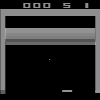
\includegraphics[width = 0.21\textwidth]{test_input_0}} 
{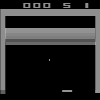
\includegraphics[width = 0.21\textwidth]{test_input_1}}\\ 
{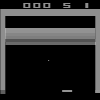
\includegraphics[width = 0.21\textwidth]{test_input_2}}
{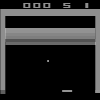
\includegraphics[width = 0.21\textwidth]{test_input_3}} 
\caption{This figure shows the input of CNN for game breakout. The function $\varphi(\cdot)$ convert the RGB(i.e. red, green, blue ) image to gray-scale image and further downsample it to four 100x100 images. The number at the upper left corner shows the current score. The number at upper middle shows the lives of the agent. The only moving object white dot is a ball. And the white bar in the middle is the agent that can reflect the ball to the bricks.}\label{function_output}
\end{figure}

\section{Deep Q Network}

After knowing the basic background and concepts of the algorithm, in this section, we combine what have been mentioned above to form a description of DQN. The arrangement of this section goes as follows. First we introduce the basic idea of DQN. Simultaneously, we introduce how is environment associated with the DQN. Then we take introduction further to formalization. There we defined the parameters in the DQN. Finally, we investigate the whole process of DQN with formalized language.

DQN was proposed by Deep Mind company in 2013, it is a really advanced algorithm for game-playing agent. It combines concepts of deep neural network and Q-learning. The DQN mimics the Q learning in a sense that it gives an action and get a reward. Based on the reward, it optimizes the parameters and make a reasonable selection of actions next time. It also mimics the behaviour of randomly selecting the a action with probability $\sigma$. This concept is from the $\epsilon$-greedy algorithm, which is also one of RL algorithm.

From previous properties, we can see that DQN has concepts from both RL and deep learning. This is why the algorithm is novel and interesting. Inspired by the applications in the field of image classification, the algorithm absorb the deep architecture as a layer of reducing the dimension and a way of extracting the information out of the image automatically.  In fact, by maintaining a set $\mathcal{D}$ and uses mini-batch optimization, the network is able to gain experiences to control the agent\cite{mnih2013playing}.

For knowing how do we use experience set $\mathcal{D}$. We need to discuss the environment, ALE provides a framework of interacting with environment of atari games . Apparently, at least the game status are parameters describing the game. The status are also the status of the RL.

For previously defined CNN, we still need to pre-process the image. According to the paper\cite{mnih2013playing}, we need to use the four stacked frames to be the one input of CNN. We describe this process by a function $\varphi(\cdot)$. Function $\varphi(\cdot)$ is defined to take four 160 x 210 pixels image as an argument and output the four greyed 80 x 80 images.

Without loss of generality we define a tuple:

$$e_t = (s_t, a_t, r_t, s_{t+1})$$ to be one-time experience of the agent where $s_t$ is a returned value by the function $\varphi(\cdot)$, $a_t$ is an action at time $t$, $r_t$ is an instant reward at time $t$.  

Then we define a set $\mathcal{D} = \{e_1, e_2, e_3, \cdots\}$ to be maintained in each iteration. As consequence, we can then use mini-batch stochastic gradient descent method to optimize the parameters of the neural network.

Specifically, as Figure~\ref{function_output} shows, $s_t$ is represented by the four down-sampled images. And as we use a very classic game breakout for testing, the actions $a_t$ in this game can only to be "moving left" or "moving right". As a consequence, the output layer for this network is set to indicate two actions. Though while playing the game, several other actions are also needed. These actions include fire(i.e. starting game) and pause for configuration purposes.  $r_t$ is defined to be only corresponded to score though it can also be related to time. But we leave that here as it belongs to the further discussion.

In the paper, it is pointed out that they have trained the neural network more than millions of iterations. 

When technical details are specified, a full functional DQN can be described. it consists following parts.

\begin{enumerate}
\item capture four screen matrices of continuous frames.
\item stack four screen matrices into a signal vector.
\item gray-scale the screen matrices.
\item linearly down-sample the screen matrices to a signal 4 x 100 x 100 vector.
\item input 4 x 100 x 100 to input layer of DQN.
\item feed-forward and get output values.
\item get reward and store $e_t$ into set $\mathcal{D}$.
\item randomly selects experiences from  $\mathcal{D}$.
\item back-propagate and train DQN.
\item store the highest output value and corresponding action
\item with a possibility $0 \leq \sigma \leq 1$, the algorithm executes action randomly otherwise executes the output action.
\item repeat from step one until it converges.
\end{enumerate}
\begin{figure}[H]
\centering
{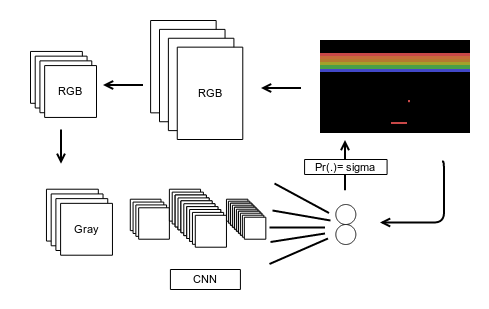
\includegraphics[width = 0.5\textwidth]{dqn}} 
\caption{This figure shows the structure of the DQN. Along with steps above, at beginning, images are preprocessed before entering the CNN and then after getting the reward,  we train the CNN with reward.}\label{dqn}
\end{figure}

\subsection{Variants}
After discussing about the whole process of DQN, we would like to consider the variants of DQN. The first thing to note is most-likely the number of layers of the CNN. Generally, if the layer of a network is increased, on one hand, the ability of approximating a function is increasing, on another hand, the difficulty of training a network is also increasing. People can only find right parameters by experience and some simple related analysis. Based on the historical experiment, 5-layers are enough to deal with the image but yet not too difficult to process. 

Another essential aspect lies in the how would the algorithm down-sample the image under this scenario. One popular down-sampling methods of CNN is the max-polling. Max-pooling means to pool the max value from a $n x n$ image piece. By doing this, the algorithm preserves the most distinctive information from the graph. Besides this method, there are also other methods e.g. linear down-sampling and random down-sampling. The mean reason of why the Max-pooling should be used is that it is a non-linear process. According to researchers' experiences\citep{lecun1998gradient}, only if the non-linear process exists, the CNN can provide some impressive result.

These variants are very important, they control how mechanisms are formed. Though more discussions can be found in LeCun's paper, here we want to give an impression that tuning each parameters in system can result a huge difference in results.

\section{Results}
In this section, we discuss the results of DQN algorithm. 

It the original paper \cite{mnih2013playing}, it is pointed out that DQN outperforms HyperNEAT for most of the tested games. In fact, for the scientific fact, the researcher also tested several other methods. Interestingly, one of method is to test performance by human.

DeepMind staff eventually used this DQN to play seven Atari games. They are Beam Rider, Breakout, Enduro, Pong, Q * bert, Seaquest and Space Invaders. While playing these games, the deep network architectures and hyper-parameter settings are exactly the same. This fully demonstrates the effectiveness of the method, and its ability of generalizing. Of course , one thing definitely modified is score. Different game score are very different resulting a lot of trouble while dealing with them . Therefore , the process of playing the game is changed. If an agent gets a positive score, the standard score will plus one and vice versa. By doing this, the testing allows the integration of different games within a framework and not leading to computational difficulties .

The Figure~\ref{result} shows the results of different algorithms. This figure is provided by the Deep Mind company\cite{mnih2013playing}.
\begin{figure}[h!]
\centering
{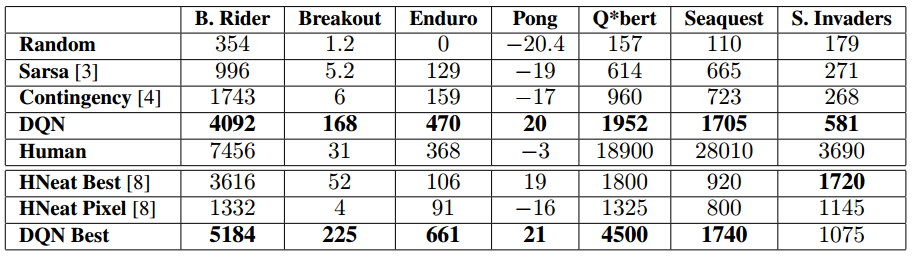
\includegraphics[width = 0.5\textwidth]{result}} 
\label{result}
\caption{This paper contains the result of the tests included in the paper "Playing Atari with Deep Reinforcement Learning" \cite{mnih2013playing}. As we can see from the figure, some famous methods are investigated. For example, State Action Reward State Action (SARSA) is one typical method in reinforcement learning and here also states the result performed by this algorithm. We can see that for a game like breakout, the DQN has impressive results. It has beaten all other method including human.}
\end{figure}
\section{Project}

In our project, we also implemented similar algorithm. 

The architecture is similar to the DQN introduced in the original paper. 

The following text lists differences.

\begin{enumerate}
\item we down-sample game screen matrices to 100 x 100 instead of 84 x 84 in pre-processing step.
\item we use 5 layers network to process the image.
\item 10 millions of iterations is too large for us. we just iterate through the network until it can behave as it apparently learns something.
\end{enumerate}

%HyperNEAT is a generative encoding that evolves the parameters and archtectures by %neuralEvolution of Augmented Topologies (NEAT) algorithm\citep{stanley2006exploiting}. It uses %a so-called Compositional Pattern-Producing Networks (CPPNs) to complete this task. CPPN %differs with current neural network in which it uses different activation functions i.e. the %function used by each neuron to regulate the value in a certain range. NEAT is an efficient %algorithm that evolve the network efficiently.

\section{Conclusions}
The RL based on deep learning architecture has shown that it can give better result in this research. In fact, it outperforms several famous algorithm in the area of RL. As a consequence, this algorithm can be very competitive in the field in RL, especially when we need to process images. 

For the sake of further discussion, we can think about why deep learning could help learning in such kind of research. The first point to mention is that this algorithm involves two processes - that is perception and control. The process of perception is the main topic in image classification. In that area, the deep architecture has been considered as state-of-the-art method. We can see this trend from the fact that in the recent years image classification competition, the deep learning are widely applied. Transforming a state-of-the-art method in other area to RL has a main problem. Unavoidably, the new method need to adopt the framework of original RL. The researchers in deep mind actually used some concept to ease the transition. For example, they used the idea of learning rate $\alpha$ , the $\epsilon$-greedy policy and the mini-batch. But besides these connections, there is nothing more related closely with transitional RL. The other area is control. In traditional RL algorithms, the action is performed by policy maintained in a list. The DQN, however, is a network, resulting the policy to be learned implicitly. This difficulty of DL is solved by the connection between the neurons of the output layer and actions space of the game. Interestingly, as we noticed the input of the algorithm is actually the four continuous down-sampled frames, the action that an agent should take at a specific time $t$ becomes an image classification problem as well.

To sum up, this algorithm DQN provides a novel way of controlling the agent under uncertain environment and it is able to outperform typical algorithms under some condition. With some drawbacks including training time and implicit policy pointed out, we need to consider the what is exactly the connection between this method and original RL.

% In the unusual situation where you want a paper to appear in the
% references without citing it in the main text, use \nocite
\nocite{langley00}
\bibliography{seminar_report}
\bibliographystyle{icml2013}
\end{document} 
% This document was modified from the file originally made available by
% Pat Langley and Andrea Danyluk for ICML-2K. This version was
% created by Lise Getoor and Tobias Scheffer, it was slightly modified  
% from the 2010 version by Thorsten Joachims & Johannes Fuernkranz, 
% slightly modified from the 2009 version by Kiri Wagstaff and 
% Sam Roweis's 2008 version, which is slightly modified from 
% Prasad Tadepalli's 2007 version which is a lightly 
% changed version of the previous year's version by Andrew Moore, 
% which was in turn edited from those of Kristian Kersting and 
% Codrina Lauth. Alex Smola contributed to the algorithmic style files.  
